% =====================================================================
%  RESULTS — revised draft (language + structural edits)
%  Reviewer-style rewrite. Unresolved factual inconsistencies are marked
%  with \todo{...} and MUST be resolved by the authors against records.
%  Requires in preamble:  \usepackage{xcolor}
%  \newcommand{\todo}[1]{\textcolor{red}{[\textbf{AUTHOR CHECK:} #1]}}
% =====================================================================

% %%%%%%%%%%%%%%%%%%%%%%%%%%%%%%%%%%%%%%%%%%%%%%%%%%%%%%%%%%%%
\section*{Results}
% %%%%%%%%%%%%%%%%%%%%%%%%%%%%%%%%%%%%%%%%%%%%%%%%%%%%%%%%%%%%

We developed a real-time, closed-loop optogenetic system to regulate population activity within a targeted cortical region monitored by wide-field calcium imaging. Trial-averaged cortical responses to optogenetic stimulation were well described by a stationary linear input--output map, providing the empirical foundation for controller design.

% ------------------------------------------------------------
\subsection*{Experimental setup and closed-loop control architecture}
% ------------------------------------------------------------
We performed closed-loop experiments in head-fixed transgenic mice co-expressing GCaMP and an inhibitory opsin, positioned in a behavioral chamber \citep{Matveev2024}. The forelimbs of each mouse rested on a freely moving wheel, and a blank screen faced the animal. We recorded neural activity at 35\,Hz using wide-field calcium imaging (Fig.~\ref{fig:figure1}A) and delivered spatially resolved optogenetic stimulation to a cortical region adjacent to the $\Delta F/F$ output kernel (Fig.~\ref{fig:figure1}B). We chose the stimulation region to overlap closely with the output kernel (Fig.~\ref{fig:figure1}C) so as to directly suppress activity within that region~\citep{Matveev2024}. In a subset of experiments, we captured motion energy from face video, defined as pixel variation squared per unit time.

\begin{figure}[h]
    \centering
    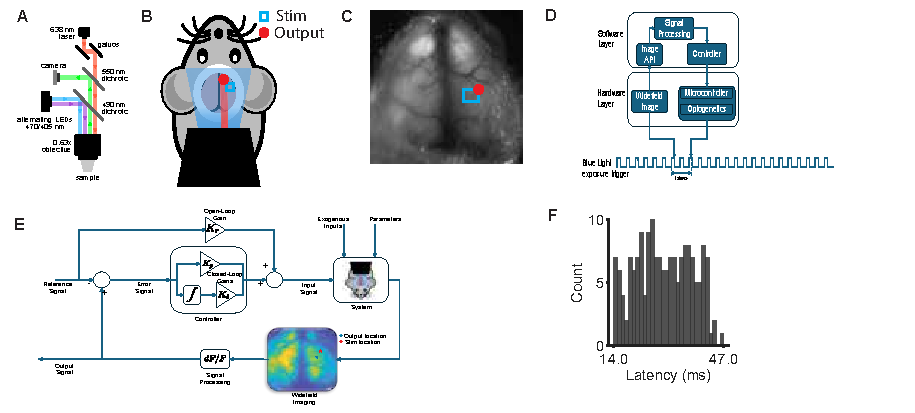
\includegraphics[width=\linewidth]{images/Figure1.pdf}
    \caption{\textbf{Experimental setup and closed-loop control architecture.}\\
    \small{
    \textbf{A:} Schematic of the wide-field microscope optical path. Blue (470\,nm) and violet (405\,nm) LEDs illuminate the dorsal cortex; emitted green photons are collected by the camera via two dichroics. A red (638\,nm) galvanometer-steered laser passes through both dichroics to deliver spatially targeted optogenetic stimulation.\\
    \textbf{B:} Schematic showing the spatial relationship between the optogenetic stimulation target (red) and the $\Delta F/F$ output region (blue box).\\
    \textbf{C:} Representative wide-field frame showing the stimulation spot (red) and the spatial kernel used as the closed-loop feedback output (blue box).\\
    \textbf{D:} Signal-flow diagram of the closed-loop pipeline. A hardware trigger initiates frame acquisition; the imaging API streams frames to the control server, which computes $\Delta F/F$ and evaluates the controller; the resulting command drives the optogenetic stimulator via a micro-controller.\\
    \textbf{E:} Block diagram of the closed-loop control architecture. The spatial-kernel $\Delta F/F$ average provides the output $y_t$; the PI controller computes a corrective input from the tracking error and sums it with the open loop component; the combined signal drives the laser.\\
    \textbf{F:} Distribution of measured end-to-end control-loop latency, of 200 loop cycles. Latency is defined as the time from camera trigger to laser-activation command, encompassing image transfer, $\Delta F/F$ computation, and digital-to-analog conversion. 
    }}
    \label{fig:figure1}
\end{figure}

We designed a hardware and software architecture for signal processing and fast closed-loop control of this mesoscale activity (Fig.~\ref{fig:figure1}D). The software layer implemented the framework required to compute the control signal from real-time feedback. Specifically, we implemented a proportional--integral (PI) feedback controller with open-loop (feedforward) compensation to drive cortical activity toward a reference $\Delta F/F$ value (Fig.~\ref{fig:figure1}E). The feedforward component supplied the nominal stimulus required to reach the reference state, computed from the calibrated controller gains, while the PI feedback component provided real-time error correction, compensating for bias arising from inaccurate feedforward gains, residual nonlinearities, and spontaneous trial-to-trial fluctuations.
% In this architecture (Fig.~\ref{fig:figure1}E), the kernel-averaged wide-field measurement serves as the system output; the controller computes an optogenetic stimulus from the error between the measured output and the reference, and this input drives the plant subject to a maximum system delay of 47ms(Fig.~\ref{fig:figure1}F). \aditya{phase limitations}
In this architecture (Fig.~\ref{fig:figure1}E), the kernel-averaged wide-field measurement serves as the system output; the controller computes an optogenetic stimulus from the error between the measured output and the reference, and this input drives the plant subject to a maximum system delay of $47$~ms (Fig.~\ref{fig:figure1}F), which sets a fundamental limit on tracking bandwidth: because a pure delay contributes a phase lag of $\omega\tau$ without attenuating gain, it accumulates a quarter cycle ($90^\circ$) of lag at $f = 1/(4\tau) \approx 5.3$~Hz and a half cycle ($180^\circ$) at $1/(2\tau) \approx 10.6$~Hz, so reference components above ${\sim}5$~Hz cannot be reliably tracked and the loop gain must fall below unity before $10.6$~Hz to preserve closed-loop stability.
% ------------------------------------------------------------
\subsection*{Trial-averaged cortical dynamics are well approximated by a linear system}
% ------------------------------------------------------------
Trial-averaged cortical responses to optogenetic stimulation followed a linear input--output map, and a low-dimensional linear time-invariant (LTI) system closely approximated both impulse and step responses. We delivered optogenetic impulse inputs at discrete amplitudes spanning 0--1.8\,mW, randomly interleaved across trials within each session. Fig.~\ref{fig:figure2}A shows the trial-averaged impulse responses for one session, from which we estimated a settling time of $\sim$200\,ms.

\begin{figure}
    \centering
    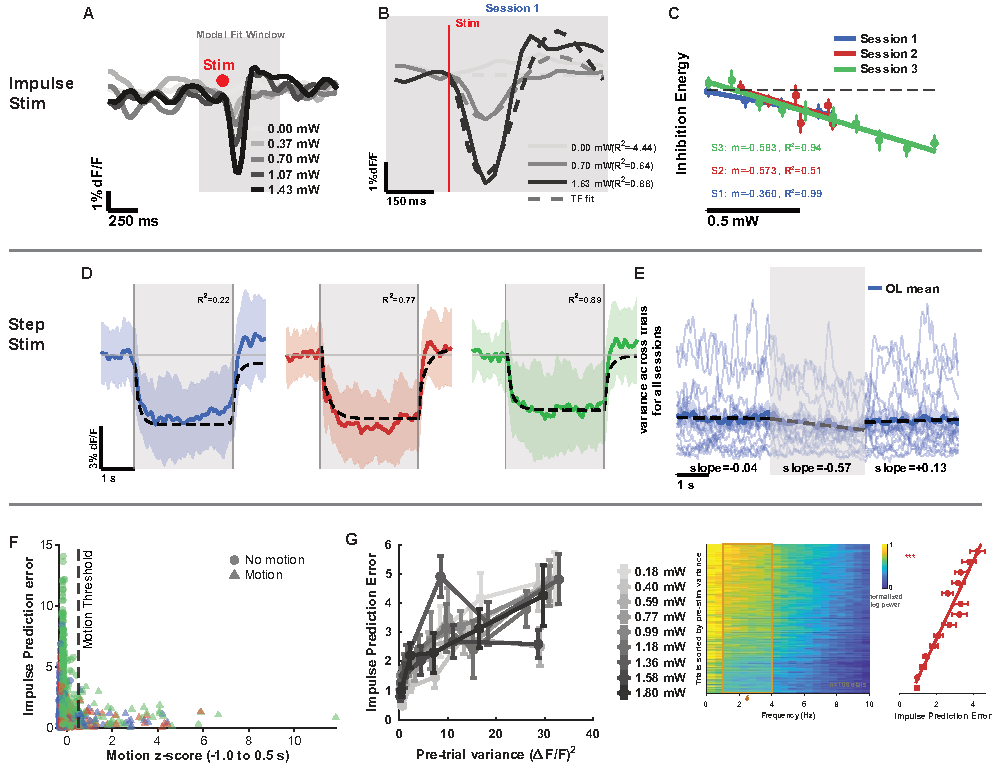
\includegraphics[width=\linewidth]{images/Figure2_extra.pdf}
    \caption{\textbf{Input--output characterization of local cortical dynamics.}\\
    \small{
    \textbf{A:} Trial-averaged $\Delta F/F$ impulse responses across five stimulation amplitudes (0--1.8\,mW; $\sim$90 trials per amplitude). Traces are aligned to stimulation onset (red line); shading shows $\pm$1\,SD across trials for the lowest and highest amplitude, bracketing the across-trial spread. Amplitude was randomly sampled on each trial.\\
    \textbf{B:} Total inhibition energy (suppression integrated over 0--200\,ms) versus stimulation amplitude for three sessions. Points show mean $\pm$ SD across trials ($\sim$50 trials per amplitude); lines show the fitted linear input--output relationship (see Materials and Methods).\\
    \textbf{C:} Predicted trial-averaged traces for three representative impulse responses. Bold traces show the trial-averaged response; dashed traces show the LTI-system fit to the trial-averaged data ($N = 90$ trials).\\
    \textbf{D:} Predicted trial-averaged traces for three representative step responses. Bold traces show the trial-averaged response; dashed traces show the LTI-system fit to the trial-averaged data ($N = 50$ trials).\\
    \textbf{E:} Across-trial variance over the trial for one representative session. Variance traces for 13 sessions are shown across the 3\,s stimulation window (gray), together with 3\,s pre- and post-stimulation windows. The bold trace is the mean across sessions; dashed lines show the linear approximation of the mean variance trace, with the fitted slope reported for the pre-, during-, and post-stimulation windows.
    }}
    \label{fig:figure2}
\end{figure}

The mean total inhibition energy per trial (see Materials and Methods) increased monotonically with stimulation amplitude and was well approximated by a linear relationship across three sessions (Fig.~\ref{fig:figure2}B; with $R^2 = 0.99, 0.51, 0.94$ and slopes $-0.36,0.57,0.58$ for three sessions). This monotonic relationship between stimulation amplitude and inhibition energy supports the design of a feedforward controller calibrated from impulse-response data \citep{astrom1995pid}. 

Step inputs applied over 3\,s trial windows produced trial-averaged trajectories that were closely approximated by an LTI system. We fit LTI systems to trial-averaged step-response data from three sessions (Fig.~\ref{fig:figure2}D) with $R^2= 0.22, 0.77,0.89$. The fitted models were low-order transfer functions consistent with the marginally stable, weakly oscillatory dynamics expected of biologically bounded cortical circuits. Session-to-session offset bias in the step response motivated the inclusion of the integral term in the PI controller (see Materials and Methods). The open-loop step stimulation also had a slight effect, reducing across-trial variance during stimulation as the stimulation period increased. We quantified this by computing the slope of across-trial variance during the stimulation window ($-0.57$), compared to near-zero slopes in the pre- and post-stimulation windows ($-0.04$ and $0.13$; $n = 13$ sessions, Fig.~\ref{fig:figure2}E). This open-loop reduction was not significant on its own, indicating that the optogenetic input did not destabilize the system; a significant, window-specific reduction in across-trial variance emerged only under closed-loop feedback, quantified by the open-loop/closed-loop variance ratio below (Fig.~\ref{fig:figure3}I).

Batch-mean $\Delta F/F$ variance during spontaneous activity decreased with trial count and stabilized beyond approximately 50 trials per session (Fig.~\ref{fig:S1}), consistent with the trial-averaging assumption (see Materials and Methods). Because variance convergence alone is a central-limit effect that does not exclude a slowly drifting mean, we additionally verified that the per-trial spontaneous mean was stationary across acquisition order: in none of the 13 sessions did the per-trial mean show a significant trend with trial index (Fig.~\ref{fig:S2}; linear regression, all $p > 0.24$; Spearman rank correlation, all $p > 0.12$), slope signs were balanced across sessions (8 positive, 5 negative; sign test $p = 0.58$), and the median session-long drift was only $0.17$ times the trial-to-trial standard deviation. The spontaneous mean is therefore stationary, supporting the zero-mean disturbance assumption that underlies the trial-averaging argument. Convergence rates differed across sessions recorded from the same region, consistent with session-to-session differences in brain state.

% ------------------------------------------------------------
\subsection*{Pre-stimulus brain state shapes predictability}
% ------------------------------------------------------------
Pre-stimulus activity affects predictability of impulse response.

% \todo{SECTION TO BE WRITTEN. Key result (prestim\_variance.m): under open-loop control, the regression slope of pre-stimulus variance against per-trial RMSE is positive (higher pre-stimulus variance $\rightarrow$ higher tracking error); under closed-loop control, the slope is near-flat, indicating that feedback decouples tracking performance from initial brain state. Add the corresponding figure reference. Then implement the Curto et al.\ (2009)-style trial-sorting analysis: split trials by pre-stimulus ($\sim$1\,s) variance into synchronized vs.\ desynchronized groups; within each group, sort trials by $|\Delta F/F|$ at $t = 0$; display $\Delta F/F$ heatmaps for open- and closed-loop conditions. NOTE: cite as Curto, Sakata, Marguet, Itskov \& Harris (2009), J.~Neurosci.\ 29(34):10600--10612 --- there is NO ``Bhatt'' or ``Issa'' author. Consider a 500\,ms or sliding pre-stimulus window, since a 1\,s window may conflate state transitions.}



% ------------------------------------------------------------
\subsection*{Closed-loop control improves reference-tracking accuracy}
% ------------------------------------------------------------
Across 13 sessions from 2 mice, with confirmed opsin expression, closed-loop feedback consistently improved tracking of a reference target activity relative to open-loop stimulation (Fig.~\ref{fig:figure3}). Under open-loop conditions, the feedforward term produced responses that systematically deviated from the reference, reflecting the inability of a fixed input to compensate for ongoing spontaneous fluctuations or for inaccuracies in the estimated open-loop controller. Under closed-loop control, the proportional term corrected instantaneous deviations, while the integral term accumulated and eliminated persistent offset, yielding substantially improved alignment with the target reference at the single-trial level (Fig.~\ref{fig:figure3}A).

\begin{figure}
    \centering
    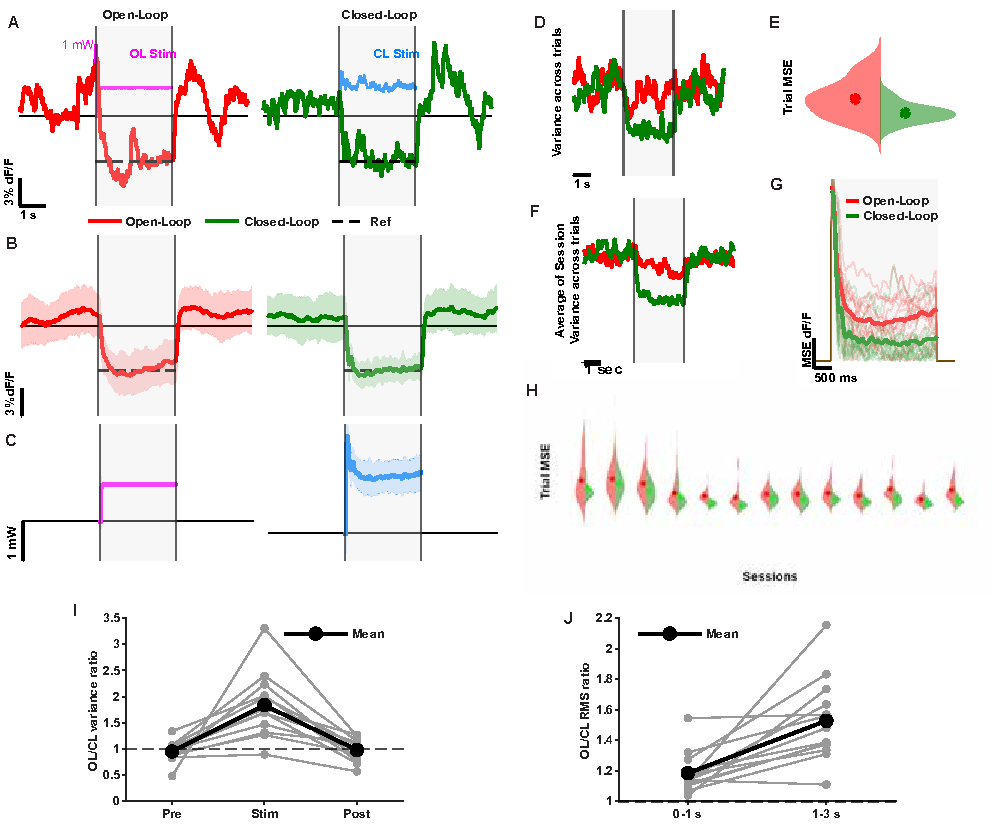
\includegraphics[width=\linewidth]{images/Figure3_extra.pdf}
    \caption{\textbf{Closed-loop versus open-loop cortical activity control} (2 mice, 13 sessions).\\
    \small{
    \textbf{A:} Single-trial example of open-loop (red) and closed-loop (green) $\Delta F/F$ responses. Gray shading marks the 3\,s stimulation window; the dashed line indicates the target $-5\%\,\Delta F/F$. Bottom traces show the corresponding optogenetic input signals.\\
    \textbf{B:} Trial-averaged $\Delta F/F$ responses under open-loop (red) and closed-loop (green) control for a representative session. Bold lines show the trial mean; thin lines show individual trials.\\
    \textbf{C:} Trial-averaged optogenetic input signals for open-loop (pink) and closed-loop (blue) conditions. Bold lines show the mean input; thin lines show individual trials.\\
    \textbf{D:} Cross-trial variance of $\Delta F/F$ as a function of time for open-loop and closed-loop conditions in a representative session. Gray shading marks the stimulation window.\\
    \textbf{E:} Distribution of per-trial tracking RMSE (root-mean-squared error over the 3\,s stimulation window, in $\%\,\Delta F/F$) for open-loop and closed-loop conditions, shown as violin plots. Points indicate individual trials.\\
    \textbf{F:} Cross-trial variance during the stimulation window, averaged across all 13 sessions, for open-loop and closed-loop conditions.\\
    \textbf{G:} Per-trial RMSE distributions pooled across all 13 sessions, shown as violin plots.\\
    \textbf{H:} Mean absolute tracking error per unit time as a function of time within the trial, averaged across all sessions (bold) with individual session traces (thin lines).\\
    \textbf{I:} Ratio of across-trial variance (open-loop / closed-loop) for each session, computed separately for the pre-stimulation window (3\,s before stimulus onset), the stimulation window, and the post-stimulation window (3\,s after stimulus offset). Gray lines show individual sessions; the bold line shows the across-session mean.\\
    \textbf{J:} Disturbance-rejection effect, shown by splitting each trial into a 0--1\,s (settling) regime and a 1--3\,s (steady-state) regime. The $y$-axis shows the ratio of open-loop to closed-loop tracking RMSE for each session. Gray lines show individual sessions; the bold line shows the across-session mean.\\
    }}
    \label{fig:figure3}
\end{figure}

Trial-averaged responses confirmed that closed-loop activity tracked the reference closely throughout the stimulation window, whereas open-loop responses showed a systematic positive bias (Fig.~\ref{fig:figure3}B). The difference in mean input between conditions (Fig.~\ref{fig:figure3}C) reflects the additional corrective signal contributed by real-time feedback. Per-trial tracking costs shifted toward lower values and showed reduced spread under closed-loop control (Fig.~\ref{fig:figure3}E), indicating both improved mean performance and greater reliability of neural modulation across trials. These improvements held across all recorded sessions (Fig.~\ref{fig:figure3}G) and required only small controller gains; for the session shown in Fig.~\ref{fig:figure3}A--E we used $K_{r} = 0.1$, $K_{p} = 0.07$, and $K_{i} = 0.1$. The sufficiency of such small gains suggests that the approximately linear, stationary input--output structure identified empirically was adequate to support stable PI feedback.

% ------------------------------------------------------------
\subsection*{Closed-loop control reduces trial-to-trial variability}
% ------------------------------------------------------------
Beyond improving mean tracking accuracy, closed-loop feedback substantially reduced trial-to-trial variability in cortical activity during the stimulation window (Fig.~\ref{fig:figure3}D). This follows from the structure of the PI controller: individual trial trajectories can be viewed as perturbations of the nominal averaged response, driven by approximately zero-mean neural disturbances and trial-to-trial brain-state fluctuations, which the controller actively steers back toward the reference, thereby compressing the cross-trial distribution of responses.

Under open-loop stimulation, response variance decreased slightly relative to the pre-stimulation baseline (Fig.~\ref{fig:figure2}E), reflecting the limited ability of the fixed feedforward term to counteract spontaneous fluctuations. Under closed-loop control, variance decreased substantially more during the stimulation window, consistent with active disturbance rejection. This reduction persisted across sessions, as confirmed by pooled within-session variance traces (Fig.~\ref{fig:figure3}D--F) and by the cross-session distribution of per-trial RMSE (Fig.~\ref{fig:figure3}G). The open-loop/closed-loop variance ratio was significantly elevated specifically during the stimulation window, but not in the pre- or post-stimulation windows (Fig.~\ref{fig:figure3}I), confirming that the variance reduction is window-specific and feedback-driven rather than a generic effect of stimulation.

The validity of these results depends on the trial-averaging assumption holding across the session; the empirical variance convergence in Fig.~\ref{fig:S1} is consistent with this assumption over the validation period. Performance varied across animals and sessions, likely reflecting residual non-stationarity in arousal and behavioral state, differences in opsin expression, and session-to-session variation in the spatial overlap between the stimulation and output regions. Despite this variability, the direction of improvement---in both tracking accuracy and trial-to-trial variance---was consistent across all experiments.

% ------------------------------------------------------------
\subsection*{Disturbance attribution: spectral and motion analysis}
% ------------------------------------------------------------
To identify what drives residual trial-to-trial tracking error, we first asked whether movement explained high-error trials and whether closed-loop feedback rejected this disturbance. Within each session we regressed per-trial tracking RMSE on concurrent motion energy, separately for open- and closed-loop trials, with RMSE z-scored within each session so that slopes were comparable across sessions ($n = 9$ sessions with simultaneous motion capture). Under open-loop control, tracking error increased with motion (median slope $+0.72$ standard-deviation units of RMSE per standard-deviation of motion; Wilcoxon signed-rank $p = 0.004$), whereas under closed-loop control this dependence was abolished (median slope $-0.02$; $p = 0.91$). The open- versus closed-loop slope difference was significant (signed-rank $p = 0.008$; the open-loop slope exceeded the closed-loop slope in 8 of 9 sessions), and within the highest motion quartile open-loop error was markedly elevated while closed-loop error remained low (rank-sum $p < 10^{-15}$; Fig.~\ref{fig:figure_motion}). Movement is therefore a principal disturbance under open-loop stimulation, and feedback control specifically rejects it, decoupling tracking accuracy from motor state.

\todo{Low-frequency spectral results to run/write: on motion-clean trials only (z-scored motion energy $\leq 1.5$), test whether elevated pre-stimulus low-frequency ($1$--$4$\,Hz) power accounts for the top-quartile high-error closed-loop trials, and report the fraction of high-error closed-loop trials coinciding with elevated low-frequency power. Absolute power $(\Delta F/F)^2$/Hz throughout. Representative low-/high-error single-trial spectra go to the supplementary figure (Fig.~S\ref{fig:lowfreq_examples}; example trials TBD by AL). Methods written in Sec.~\ref{sec:disturbance}.}

\begin{figure}[h]
    \centering
    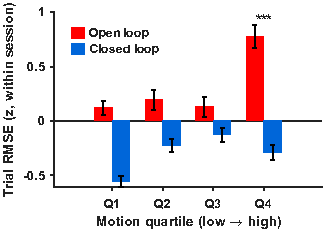
\includegraphics[width=0.5\linewidth]{images/motion_mse_quartile.pdf}
    \caption{\textbf{Closed-loop feedback rejects movement-driven disturbance.}
    Per-trial tracking RMSE (z-scored within session) binned by concurrent
    motion-energy quartile (low~$\rightarrow$~high), for open-loop (red) and
    closed-loop (green) trials pooled across 9 sessions with motion capture.
    Error bars show SEM. Open- and closed-loop error are comparable at low
    motion but diverge sharply in the highest motion quartile, where open-loop
    error rises while closed-loop error stays low (rank-sum $p < 10^{-15}$).}
    \label{fig:figure_motion}
\end{figure}

% ------------------------------------------------------------
\subsection*{Feedback rejects a state-dependent disturbance carried by the contralateral hemisphere}
% ------------------------------------------------------------
Because the two hemispheres are strongly co-active, spontaneous activity in the stimulated (ipsilateral) region is well predicted from the opposite hemisphere. We fit a stimulation-blind linear predictor from contralateral pixels to the ipsilateral control readout on spontaneous, no-laser epochs; it generalized to held-out pre-stimulus windows (contralateral$\rightarrow$ipsilateral $R^2 = 0.85$ open loop and $0.89$ closed loop; representative session), giving a trial-by-trial readout of the ongoing brain state the controller must contend with.

We first asked, at the level of the whole trial, whether this pre-stimulus state predicts the outcome. Using the level of the contralateral-derived prediction in the second before stimulation as the state, the magnitude of the actual ipsilateral response over the steady-state window (1--3\,s) scaled steeply with state under open loop but was nearly flat under closed loop (Fig.~\ref{fig:figure4}A; bootstrap open$-$closed slope difference \todo{[$\Delta$slope; $p$]}). Feedback thus decouples the trial outcome from the ongoing brain state that otherwise sets it.

To identify which state factors drive residual error, we regressed per-trial tracking error (RMSE) on the initial deviation, the motion energy, and the relative 2--4\,Hz (delta) power---the same state variables and windows used in Fig.~\ref{fig:figure_motion}. Beyond the initial deviation, motion and delta power each explained additional error variance \todo{[$\Delta R^2$ per factor; $n$ sessions]}, identifying movement and low-frequency state as the dominant disturbance sources (Fig.~\ref{fig:figure4}B).

We then resolved the mechanism at the single-trial level. Applying the predictor on every stimulation trial defines the \emph{Global} component $G$---the activity the ipsilateral region would have shown with no controller input, that is, the disturbance---and the \emph{Local} component $L = A - G$, the effect of the laser and controller on top of it (Fig.~\ref{fig:figure4}C). Across trials the actual response was well reconstructed as the Global disturbance plus the average local response (cross-validated $R^2 = 0.85$ open loop, $0.78$ closed loop), confirming that $A = G + L$ captures the single-trial response. Treating $G$ as a zero-referenced, time-varying disturbance and the tracking error as $E = A - r$ (reference $r = -5\%\,\Delta F/F$), we quantified per-trial disturbance rejection as the ratio $\rho = \lVert E\rVert/\lVert G\rVert$ over the steady-state window, where $\rho = 0$ denotes perfect rejection and $\rho = 1$ a disturbance that passes unattenuated. Closed-loop control rejected substantially more of the disturbance than open loop (median $\rho$ \todo{[OL] vs [CL]}, rank-sum \todo{$p$}; Fig.~\ref{fig:figure4}C), and this held across sessions \todo{[$n$ sessions; signed-rank $p$]}.

Finally, we asked whether this fine-grained rejection itself depends on the state entering each trial. Binning trials by pre-trial motion energy and by relative delta power, rejection degraded in high-motion and high-delta states under open loop but was more state-robust under closed loop (Spearman \todo{$r_s$ [OL] vs [CL]}; Fig.~\ref{fig:figure4}D,E). The controller therefore behaves as an internal model that estimates and cancels a disturbance shared across the cortex, making reference tracking robust to the fluctuating brain state that otherwise dominates open-loop error.

\begin{figure}[h]
    \centering
    % \includegraphics[width=\linewidth]{images/Figure4.pdf}  % panels pending cross-session sweep + paperStyle
    \caption{\textbf{Closed-loop feedback decouples the controlled response from a state-dependent disturbance carried by the contralateral hemisphere.}\\
    \small{Representative session (AL\_0033, 2025-02-26); open loop red, closed loop blue; rejection $\rho$ over the 1--3\,s steady-state window ($\rho = 0$ perfect rejection, $\rho = 1$ disturbance passes unattenuated).\\
    \textbf{A:} Trial-average state dependence. Pre-stimulus state (level of the stim-blind contralateral-derived prediction) versus the magnitude of the actual ipsilateral response over 1--3\,s; open loop scales steeply with state, closed loop is flat (bootstrap open$-$closed slope difference).\\
    \textbf{B:} Error-contribution model. Per-trial tracking error (RMSE) regressed on initial deviation, motion energy, and relative 2--4\,Hz power; $\Delta R^2$ of each factor over the base model.\\
    \textbf{C:} Residual decomposition and rejection. The controlled response $A$ splits into the Global disturbance $G$ (predicted from the contralateral hemisphere with no controller input) and the Local component $L = A - G$ (laser and controller effect), shown on one representative trial; per-trial rejection $\rho = \lVert A-r\rVert/\lVert G\rVert$ (1--3\,s) is lower in closed loop.\\
    \textbf{D:} $\rho$ by pre-trial motion-energy quartile (low~$\rightarrow$~high) and \textbf{E:} by relative 2--4\,Hz power quartile, open and closed loop.}}
    \label{fig:figure4}
\end{figure}

\todo{Single-session draft (m4 = AL\_0033 2025-02-26). Panel sources: A \texttt{ctrl\_state\_dependence.m} ($s\_lvl\rightarrow o\_act$, bootstrap OL$-$CL slope); B \texttt{cl\_mse\_factors.m} / \texttt{cl\_rmse\_factor\_windows.m} ($\Delta R^2$ waterfall); C--E \texttt{internal\_model\_principle.m} (\texttt{[IMP-REJECT]}, \texttt{[IMP-STATE-QUARTILE]}). Fill panel-A slopes, panel-B $\Delta R^2$, panel C--E medians/slopes and all cross-session statistics from the Stage 1$\rightarrow$2 cross-session sweep; assemble \texttt{Figure4.pdf} at paperStyle once the sweep is done. Supplementary: contra$\rightarrow$ipsi predictor CV-$R^2$ validity + distributed contralateral co-suppression (\texttt{stim\_network\_coupling.m}) support treating $G$ as a shared-network disturbance.}

% ------------------------------------------------------------
\subsection*{Feedforward control for variable reference tracking}
% ------------------------------------------------------------
Feedback and preview correct different failures of sinusoidal tracking: feedback removes trial-to-trial variability, while preview removes the phase lag imposed by the plant. We asked the controller to track a 1\,Hz sinusoidal reference for 4\,s in a dual-opsin mouse (AL\_0048, right hemisphere, inhibitory opsin), and crossed two factors in a $2\times2$ design---feedback on or off, and preview on or off---giving four modes: open-loop (OL), open-loop with preview (OL$+$p), closed-loop (CL), and closed-loop with preview (CL$+$p). The preview block shifts the reference forward by a fixed lookahead before it reaches the controller, compensating the delay of the cortical response rather than its amplitude (Fig.~\ref{fig:figure5}A). We report one representative session in detail (200 sinusoidal trials; $n = 51, 46, 46, 57$ trials for OL, OL$+$p, CL, CL$+$p) and the consistency of each effect across three sessions.

Open-loop tracking followed the reference in shape but lagged it and drifted between trials (Fig.~\ref{fig:figure5}B,C). Adding feedback reduced per-trial tracking error: median RMSE fell from $3.82$ to $2.80$\,\%\,$\Delta F/F$ between OL and CL (rank-sum $p = 7.7\times10^{-4}$; Fig.~\ref{fig:figure5}G), and across-trial variance fell from $17.9$ to $14.8$ (Fig.~\ref{fig:figure5}E). The same ordering held in every session tested (CL $<$ OL for both RMSE and variance in 3/3 sessions; Fig.~\ref{fig:figure5}I,K), and pooling per-trial RMSE across sessions confirmed it (OL $4.58 \pm 1.77$, $n = 136$; CL $3.83 \pm 1.94$, $n = 100$; rank-sum $p = 1.5\times10^{-4}$; Kruskal--Wallis across all four modes $\chi^2 = 19.6$, $p = 2.1\times10^{-4}$). A repeated-measures test treating session as the unit is underpowered at $n = 3$ and did not reach significance (Friedman $p = 0.060$), so we treat the direction, not the session-level test, as the result.

Preview cancelled the phase lag but did not by itself improve tracking error. The cortical response lagged the reference by $60^\circ$ under open loop and by $36^\circ$ under closed loop; adding preview moved both to approximately zero ($5^\circ$ and $-9^\circ$ respectively; Fig.~\ref{fig:figure5}H). The correction matched the lookahead by construction: a five-sample preview at 35\,Hz corresponds to $143$\,ms, or $51^\circ$ at the 1\,Hz drive frequency, and the measured open-loop correction across all pooled trials was $5.0$ samples ($51.4^\circ$, median). Lag cancellation replicated in all three sessions (Fig.~\ref{fig:figure5}J). Tracking error, however, was unchanged by preview (OL versus OL$+$p, median RMSE $3.82$ versus $3.55$, $p = 0.32$; pooled across sessions $p = 0.44$), and preview did not further improve closed-loop error (CL versus CL$+$p, $p = 0.093$). Closed-loop control with preview did reduce error relative to open loop ($p = 0.020$) and produced the tightest distribution of the four modes (SD $1.57$ versus $1.85$, $2.75$ and $2.19$ for OL, OL$+$p and CL), but the error reduction is attributable to feedback and the lag correction to preview.

Decomposing the error clarifies why the two mechanisms do not overlap. Because the stimulation window contains exactly four cycles of the drive, per-trial squared error partitions without loss into a constant-offset term, a term at the drive frequency, and the remaining broadband term. Averaged over the three sessions, preview reduced the error at the drive frequency roughly threefold in every comparison (OL $3.14 \rightarrow$ OL$+$p $0.89$; CL $1.78 \rightarrow$ CL$+$p $1.22$\,(\%\,$\Delta F/F)^2$), while feedback reduced the broadband term ($10.55 \rightarrow 6.62$ from OL to CL). Preview therefore acts on the component of error that a fixed phase relationship can remove, and feedback on the component generated by ongoing spontaneous activity. Closed-loop control with preview was the only mode to engage both, and had the lowest total error power in two of three sessions.

\begin{figure}
    \centering
    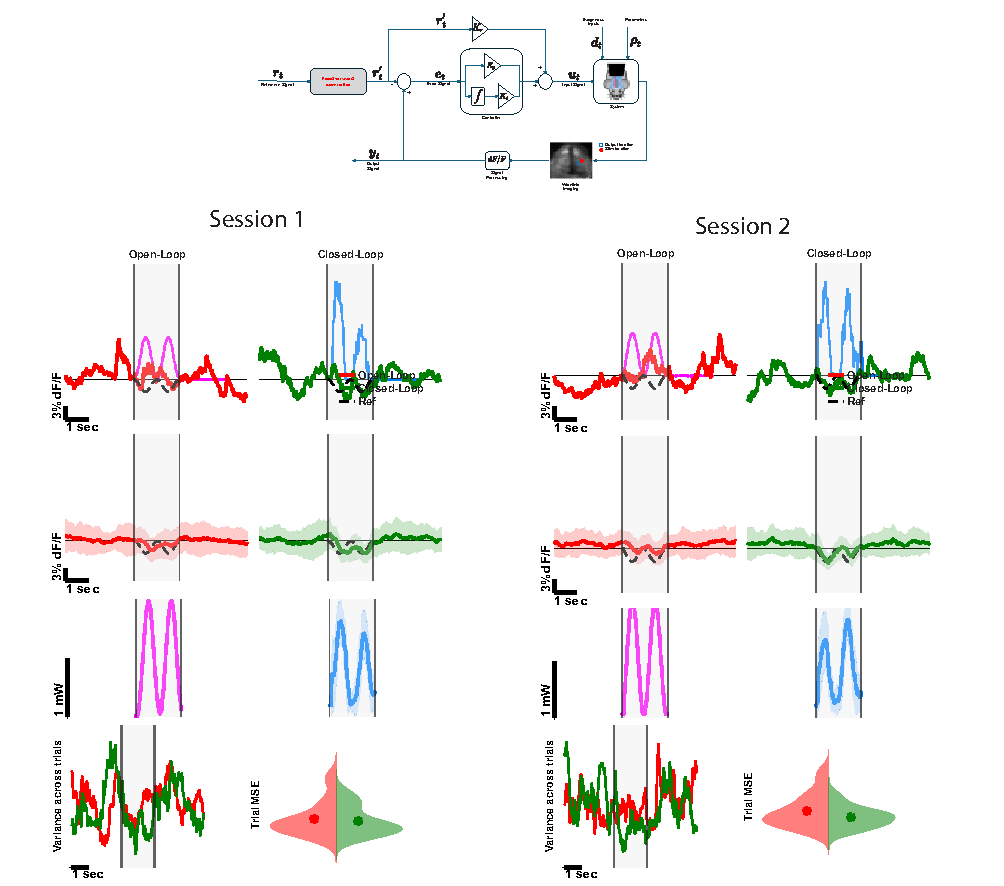
\includegraphics[width=0.82\linewidth]{images/Figure5.pdf}
    \caption{\textbf{Feedback and preview correct different failures of sinusoidal reference tracking.}\\
    \small{
    All panels: AL\_0048, right hemisphere (inhibitory opsin), 1\,Hz sinusoidal reference, 4\,s stimulation window. Four modes throughout: open-loop (OL, red), open-loop with preview (OL$+$p, orange), closed-loop (CL, blue), closed-loop with preview (CL$+$p, green). Grey traces are the delivered laser command, black dashed traces the reference.\\
    \textbf{A:} Controller architecture; a preview block shifts the reference forward by a fixed lookahead before it reaches the PI controller.
    \textbf{B:} One representative trial per mode; vertical lines and shading mark the stimulation window.
    \textbf{C:} Trial average $\pm$ SD ($n = 51, 46, 46, 57$ trials).
    \textbf{D:} Trial-average laser command $\pm$ SD, in mW; panels B--D share the time axis carried by D.\\
    \textbf{E:} Across-trial variance over time. \textbf{F:} RMSE over time, mean $\pm$ SEM (bands are asymmetric because mean and edges are square-rooted after averaging squared error).\\
    \textbf{G:} Per-trial RMSE by mode: half-violins show the full distribution (density estimated in log space), dots are individual trials, bars are median and interquartile range. The axis is logarithmic so that no trial is clipped. $^{*}p<0.05$, $^{***}p<0.001$, Wilcoxon rank-sum.
    \textbf{H:} Phase lag relative to the reference from a 1\,Hz fundamental fit to the trial average; dashed line marks the preview lookahead ($51^\circ$ at 1\,Hz).\\
    \textbf{I--K:} Consistency across three sessions---one point per session per mode joined by faint lines, bold bar the across-session mean---for per-trial RMSE (I), phase lag (J) and across-trial variance (K). Controller gains, reference amplitude and delivered optical power differ between sessions, so I--K report direction and consistency, not magnitude.\\
    }}
    \label{fig:figure5}
\end{figure}


